% 
%\subsection{Impacto del tamaño del set de entrenamiento}%
%\label{sub:exp_training_set}

% TL;DR; Como se diseño el experimento
%
Fueron tomadas mediciones sobre el comportamiento del \textit{accuracy} al
reducir el tamaño del set de entrenamiento para \knn{} con PCA.\@ Para ello se
redujo el tamaño muestral, tomando distintas sub-muestras al azar, respetando
una proporción pareja entre reseñas con calificación positiva y negativa.
% k y alpha
Se mantuvieron constantes $k$ y $\alpha$. El experimento se repitió para
distintas configuraciones de los mismos.

% acc vs N; k fijo; distintos alpha
\begin{figure}[ht]
    \centering
    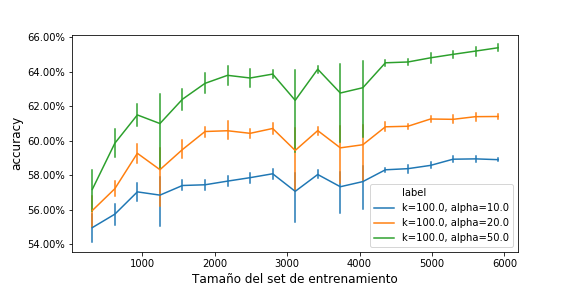
\includegraphics[width=0.6\textwidth]{img/exp_subsampling_k_fijo}
    \caption{\textit{Accuracy} obtenido al reducir el conjunto de
    entrenamiento.  Para valor fijo de $k=100$.}%
    \label{fig:subsampling_k_fijo}
\end{figure}

% acc vs N; alpha fijo; distintos k
\begin{figure}[ht]
    \centering
    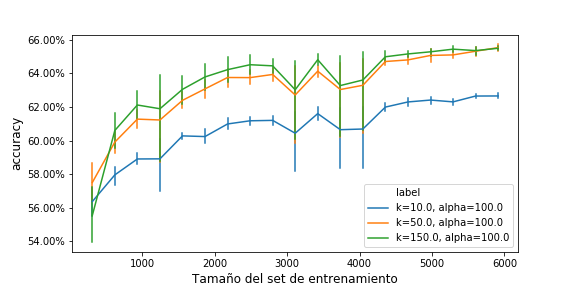
\includegraphics[width=0.6\textwidth]{img/exp_subsampling_alpha_fijo}
    \caption{\textit{Accuracy} obtenido al reducir el conjunto de
    entrenamiento.  Para valor fijo de $\alpha=100$.}%
    \label{fig:subsampling_alpha_fijo}
\end{figure}

% TL;DR; mas data => mas accuracy.
%
Puede observarse en las figuras~\ref{fig:subsampling_k_fijo}
y~\ref{fig:subsampling_alpha_fijo} que el \textit{accuracy} incrementa al
incrementar el tamaño muestral.  Por otro lado, la calidad del modelo crece
cada vez en menor medida, por lo que se cree que existe un punto a partir del
cual carece de sentido práctico incrementar el set de entrenamiento. Como el
rendimiento del modelo sigue siendo bajo, creemos que la máxima cantidad de
instancias de entrenamiento disponible, $N = 6225$, esta por debajo del tamaño
óptimo.

% TL;DR; El tamaño óptimo parece ser independiente de k y alpha.
%
Se observó el mismo comportamiento de la curva para todas las configuraciones
de $k$ y $\alpha$, por lo que se cree, el tamaño muestral óptimo es
independiente de los hiperparámetros a escoger.

% TL;DR; Se observa mayor varianza para N bajo.
%
A su vez se observa que la varianza en el \textit{accuracy} es mayor para
tamaños muestrales chicos. Esto es porque las reseñas conocidas por el modelo
pueden ser, con mayor probabilidad, poco representativas la totalidad de las
reseñas.
